\documentclass[a4paper,12pt,twoside,openright]{memoir}

\newcommand{\subject}{From Existing Software to Models}

%%%% PACKAGES %%%%

\usepackage[T1]{fontenc}
\usepackage[utf8]{inputenc}
\usepackage{fourier}
\usepackage[english]{babel}

\usepackage{graphicx}
\graphicspath{{Images/}}

\begin{document}

\chapter{Process Analyse}

    \section{Beskrivelse - Hvad gjorde vi i P1} 

        \subsection{Projektplanlægning}
I hvilket omfang har gruppens medlemmer haft samme opfattelse af hvad projektplanlægning indebærer? Har I haft nogle projektplaner? I så fald: Hvilke, hvad har I anvendt dem til og hvordan har de fungeret? Hvis ikke: Vil I lave projektplaner i P1? I så fald: Hvilke og hvad vil I bruge dem til?\newline


Inden for den første uge af P1, lavede vi en tids plan for P1, tids blev lavet en tidsplan(ses her under) med poster så der let kunne laves om, eller flyttes rundt på emnerne, hvis vi havde brug for mere tid eller hvis et emne blev færdigt. Hen i slutningen af Projektet blev der lavet  en tidsplan v. 2.0. vores arbejde, er blevet udarbejdet  efter tidsplanen, for at kunne have et overblik over hvad der skulle laves og hvornår det skulle være færdigt.


            \begin{figure}[ht!]
                \centering
                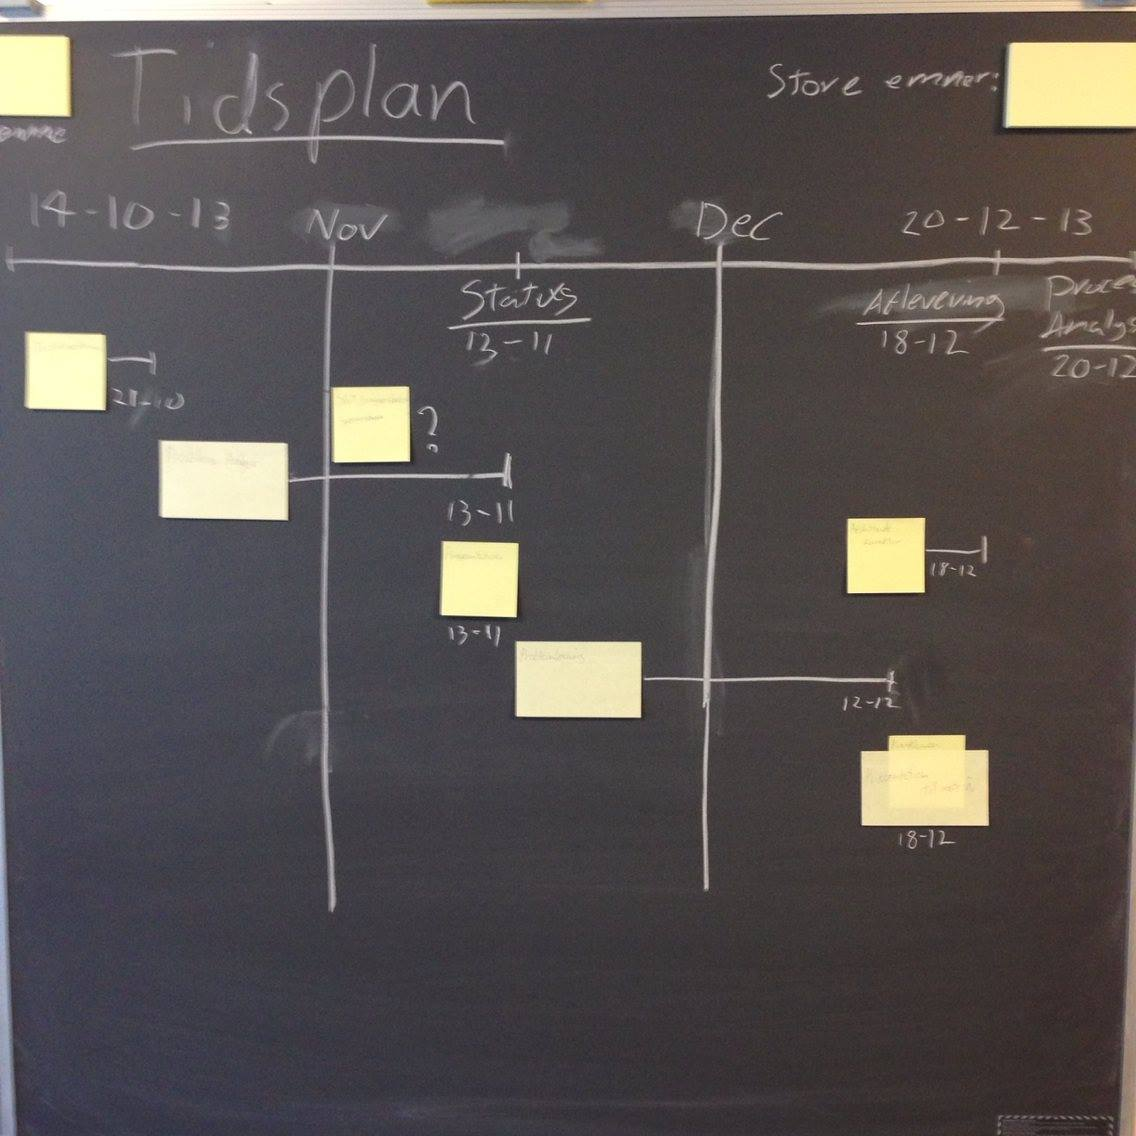
\includegraphics[width=0.5\textwidth]{Images/9.jpg}
                \caption{BAH}
                \label{4}
            \end{figure}

            \begin{figure}[ht!]
                \centering
                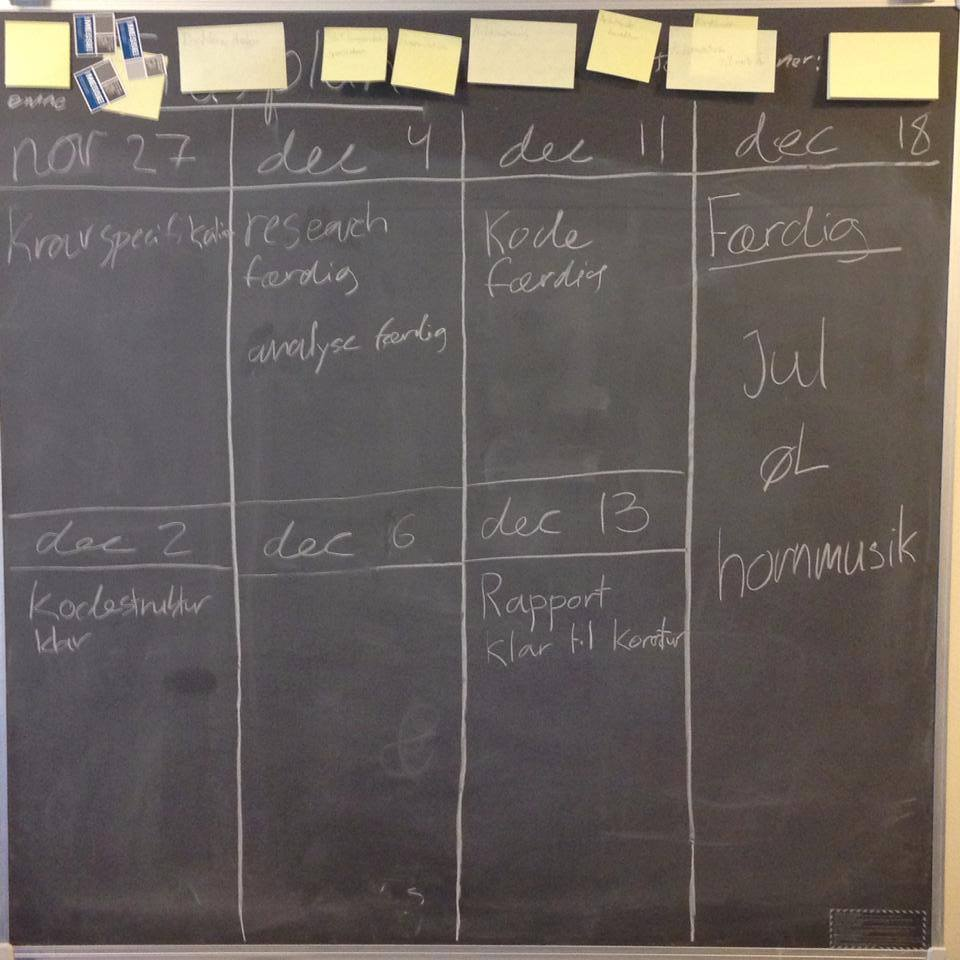
\includegraphics[width=0.5\textwidth]{Images/2.jpg}
                \caption{BAH}
                \label{4}
            \end{figure}

        \subsection{Gruppesamarbejde}

Har I lavet en samarbejdsaftale (mundtlig/skriftlig)? Hvorfor/Hvorfor ikke?\newline

Der blev lavet en samaarbejdsaftale inden for den første uge i P1, hvor alle var med til at komme med input og bagefter blev der skrevet under af alle medlemmer af gruppen.\newline

Hvor tit har I holdt møder?\newline

Der blev/bliver holdt møde hver morgen, for at hører hvor langt folk er med den opgave de er blevet stillet og for at få en samlet oversigt over de emener som er påbedyndt og hvilke emener som mangler i Tidsplanen. Under de daglige møde blev der lavet en dag-til-dag tidsplan for hvilke emener vi skulle lave og hvad der skulle skrives.\newline

Hvad gjorde I hvis en person kom for sent/ikke kom til møderne?\newline

I samarbejds aftalen, er det aftalt af hvis man kommer forsent skal man medbringe noget "consumable" til gruppen. I aftalen står der os at hvis man kommer for sent skal det meldes til mindst to af gruppen medlemmer.\newline

Hvordan har I afviklet møderne? (F.eks. med mødeleder, via runder om bordet, fri diskussion etc.)\newline

Når vi har haft møder, har vores gruppe udarbejdet en "Finger metode" så når man vil sige noget både under møder og disskusioner, hvis man er den første der vil sige noget efter Ham/Hende som har ordet rækker man 1 finger i luften. Hvis man er nr. 2, rækker man to finger i luften ovs.\newline

Hvordan har kommunikationen været i jeres gruppe? Var der nogen, der talte hele tiden? Var der nogen, der aldrig sagde noget?\newline

Alle har kunne give input til alle diskusioner og møder, men inputtet er hovedet salig kommet fra de personer som har haft viden inden for det  emne som blev diskuteret under mødes.\newline

Hvordan har motivationen været hos de enkelte gruppemedlemmer?\newline

Har I oplevet problemer med forskelle i motivation? I så fald: Hvad har I gjort for at løse problemerne?\newline

Hvordan sikrede I konstruktiv kritik af hinandens arbejdsblade til rapporten?\newline

        \subsection{Hvordan arbejder vi og hvorfor}

Efter hvilke kriterier har I fordelt arbejdsopgaverne mellem jer? Har det fungeret tilfredsstillende for alle?\newline

Vores gruppe har primært arbejdet i små gruppere, fordi vi mener at for mange på en opgave ikke nødvendigvis giver bedre resultat og da gruppen regelmæssig diskutere om forskellige emner, har det været en god ide at lave så grupper så en diskussion ikke har stoppet alt arbejdet, men alt har været snakket igennem i gruppen, selvom vi har arbejdet i mindre grupper.\newline

            \begin{figure}[ht!]
                \centering
                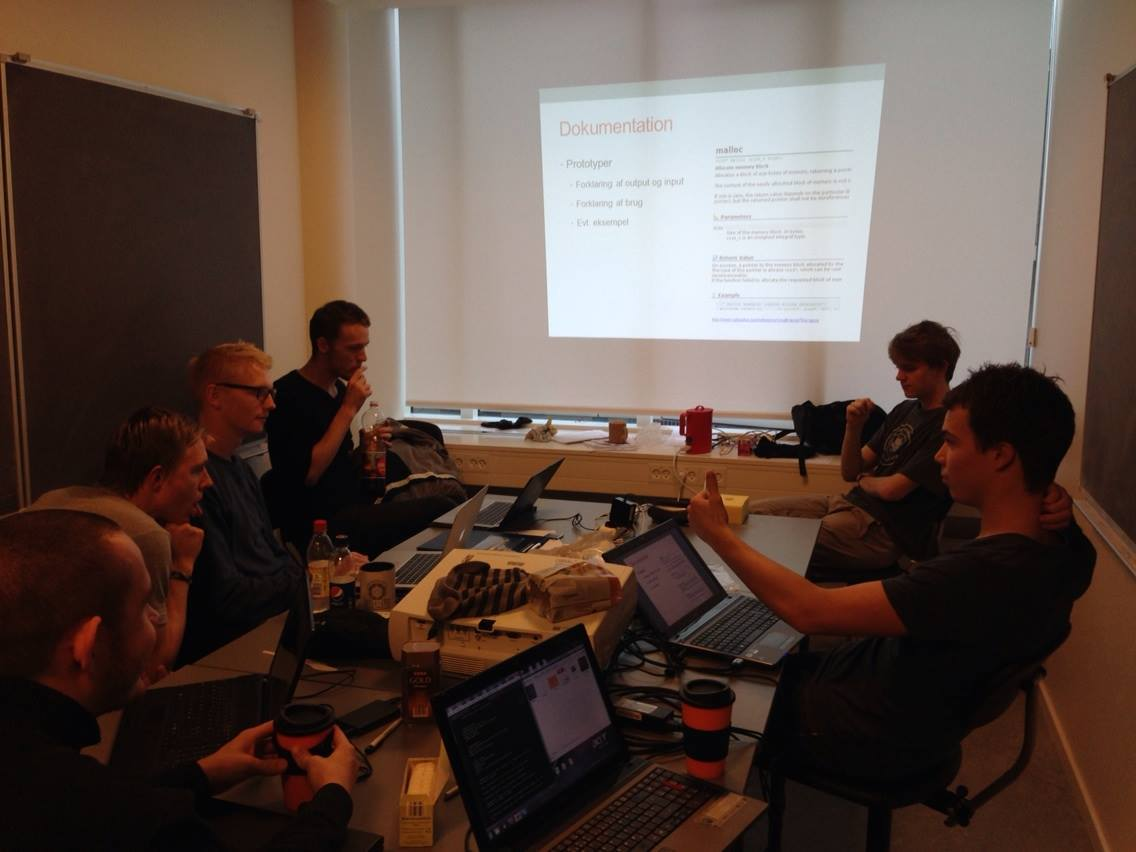
\includegraphics[width=0.5\textwidth]{Images/8.jpg}
                \caption{BAH}
                \label{4}
            \end{figure}

            \subsection{Belbin rolle fordeling og grupper}

I gruppen har vi under projekt arbejde og materiale søgning arbejde i små grupperr, hvor vi har arbejdet ud fra belbin arbejds model, hvor vi har lavet  gruppen så mindst et medlem har stor viden inden for emnet eller programering, så denne person kunne forklarer og vise hvordan han har løst opgaven. Når vi har lavet grupperog fordelt arbejdet, har vi sat nogle emner op på det der skal laves og folk har kunne vælge dem de ville arbejde med og dermed delt os i små grupper, så vi har kunne lave flere ting på en gang, men hver dag har vi lavet gruppe møde på hvad der er blevet laver  og hvor langt de enkelte grupper er. Efter gruppe arbejde har vi snakket  om det i hele  gruppen, og givet  hinanden kontroktiv kritik.\newline
         
            \subsection{Diskussion}

Brugte gruppen uforholdsvis lang tid på diskussioner? Hvorfor?\newline

Når vi har valgt at arbejde i små grupper,har vi også været ude for at skulle diskutere noget, diskussion har startet i den lille gruppe er blevet diskuteret vidre i hele gruppen så alle er kommet med input og de positive og negative sider og blevet vendt.\newline

            \subsection{Samarbejde med vejlederen}

Har I haft en samarbejdsaftale med jeres vejleder? I så fald: har den fungeret tilfredsstillende?\newline

Vores hoved vejleder er: Rikke Hagensby Jensen, i starten af P1 blev der lavet en Samarvejdsaftale med vejlederen. Som beskriver: Vejledermøder, Korrespondance og Læsemateriale til P1.\newline

Hvordan forberedte I møder med jeres vejleder?\newline

Til vejledermøderne blev der lavet en dagsorden af gruppen, som blev fuldt under mødet. dagsordenen, kunne indeholde punkter som: spørgsmål fra vejleder, spørgsmål til vejleder, respon til gruppen fra report, vider forløb og aftal næste møde.\newline

Hvilken type vejledning ønskede I fra vejlederen?\newline Hvilken type vejledning fik I?\newline

        \section{Problemformuleringer}

Hvordan lavede I indledning til problemformuleringen?\newline

        \subsection{Brainstorm}
        
I starten af forløbet, lavede i brainstorm på tavlen, hvor vi delte det op i 3 store  emner, "Indoor navigation", "Problemer der skal håndteres" og "Intressenter". Disse emner blev delt ind i under emner, hvor vi smed relevante problemer og emner op omkring navigation eller SOTA som kan buges til navigation.\newline

        \begin{figure}
        \centering
            \begin{minipage}{0.45\textwidth}
                \centering
                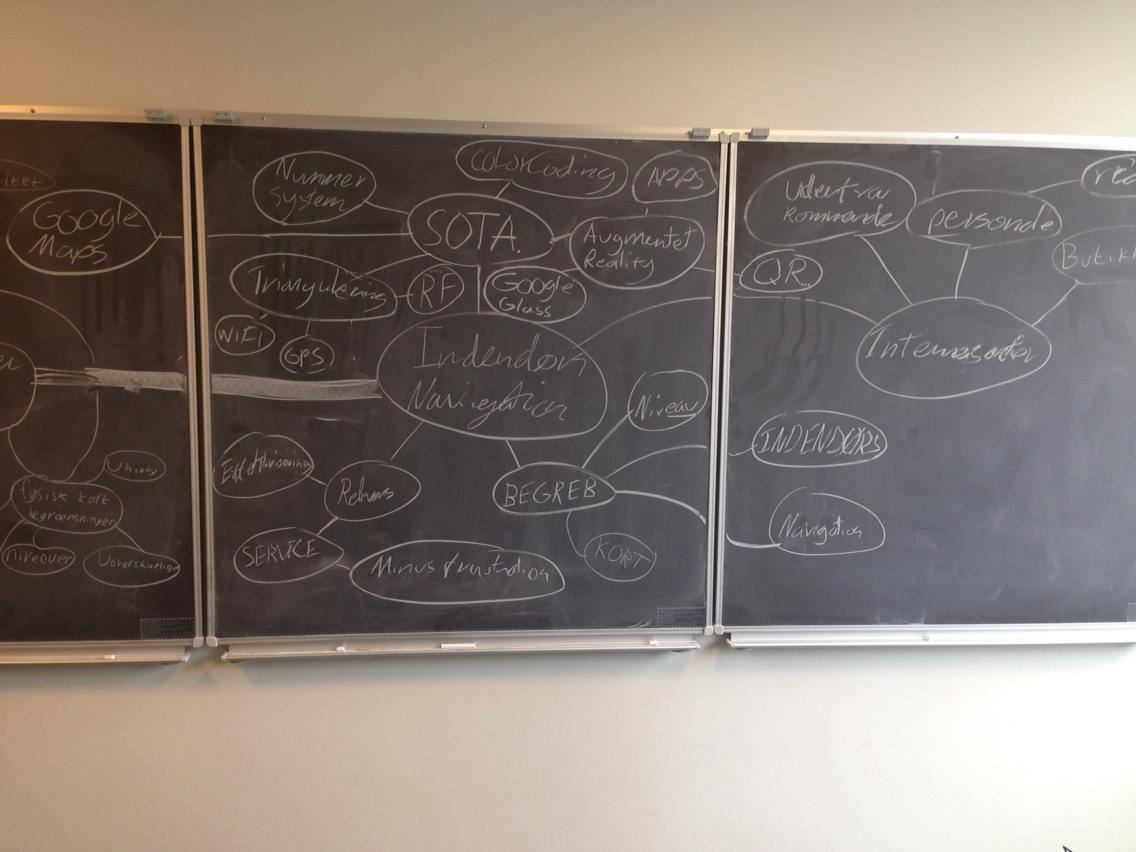
\includegraphics[width=\textwidth]{Images/1.jpg}
                \caption{BAH}
                \label{4}
            \end{minipage}
            \begin{minipage}{0.45\textwidth}
                \centering
                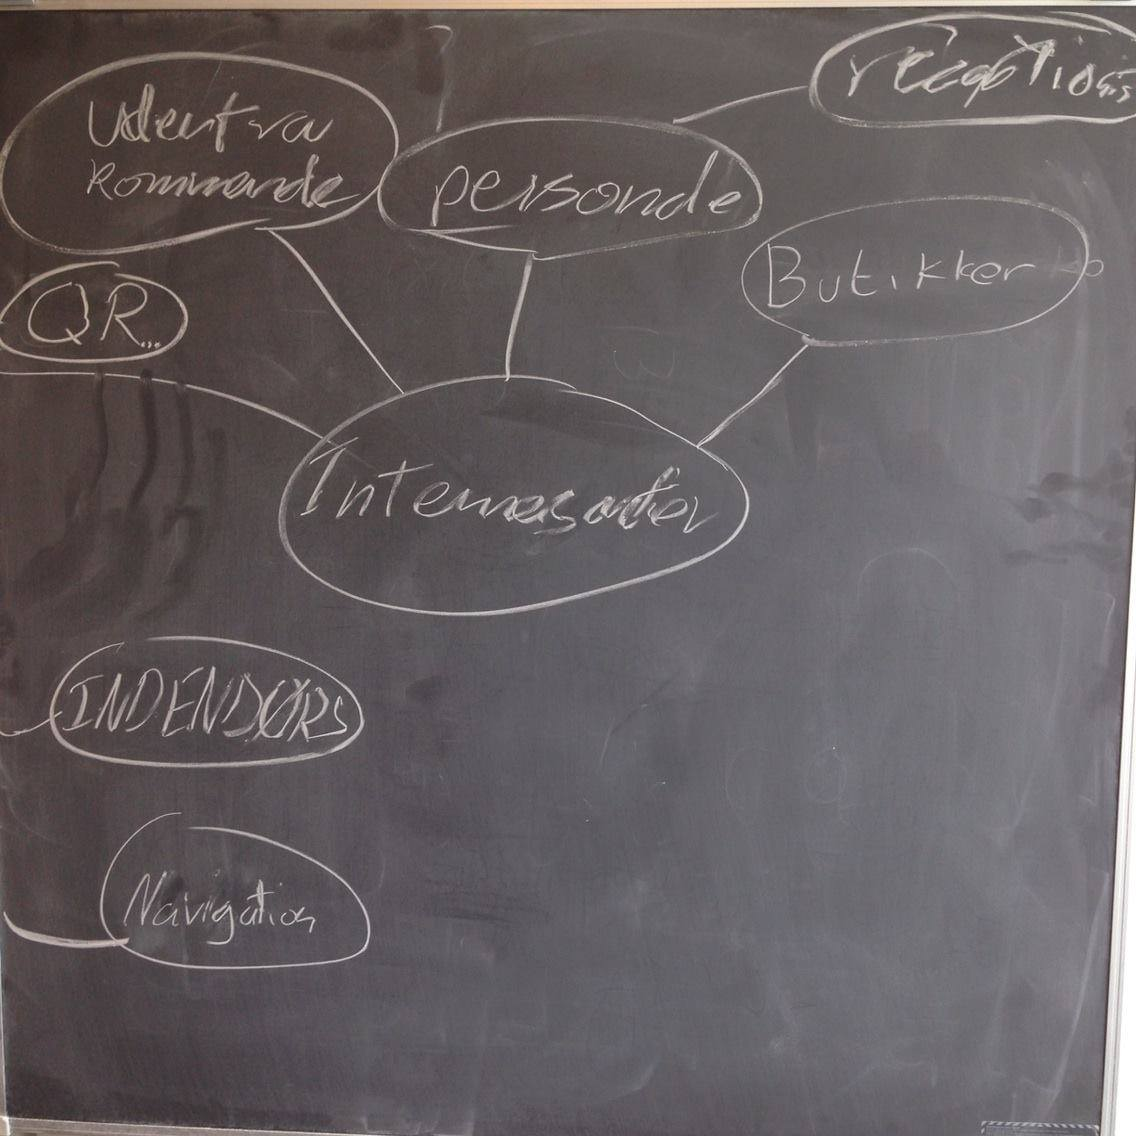
\includegraphics[width=\textwidth]{Images/3.jpg}
                \caption{BAH}
                \label{4}
            \end{minipage}
            \begin{minipage}{0.45\textwidth}
                \centering
                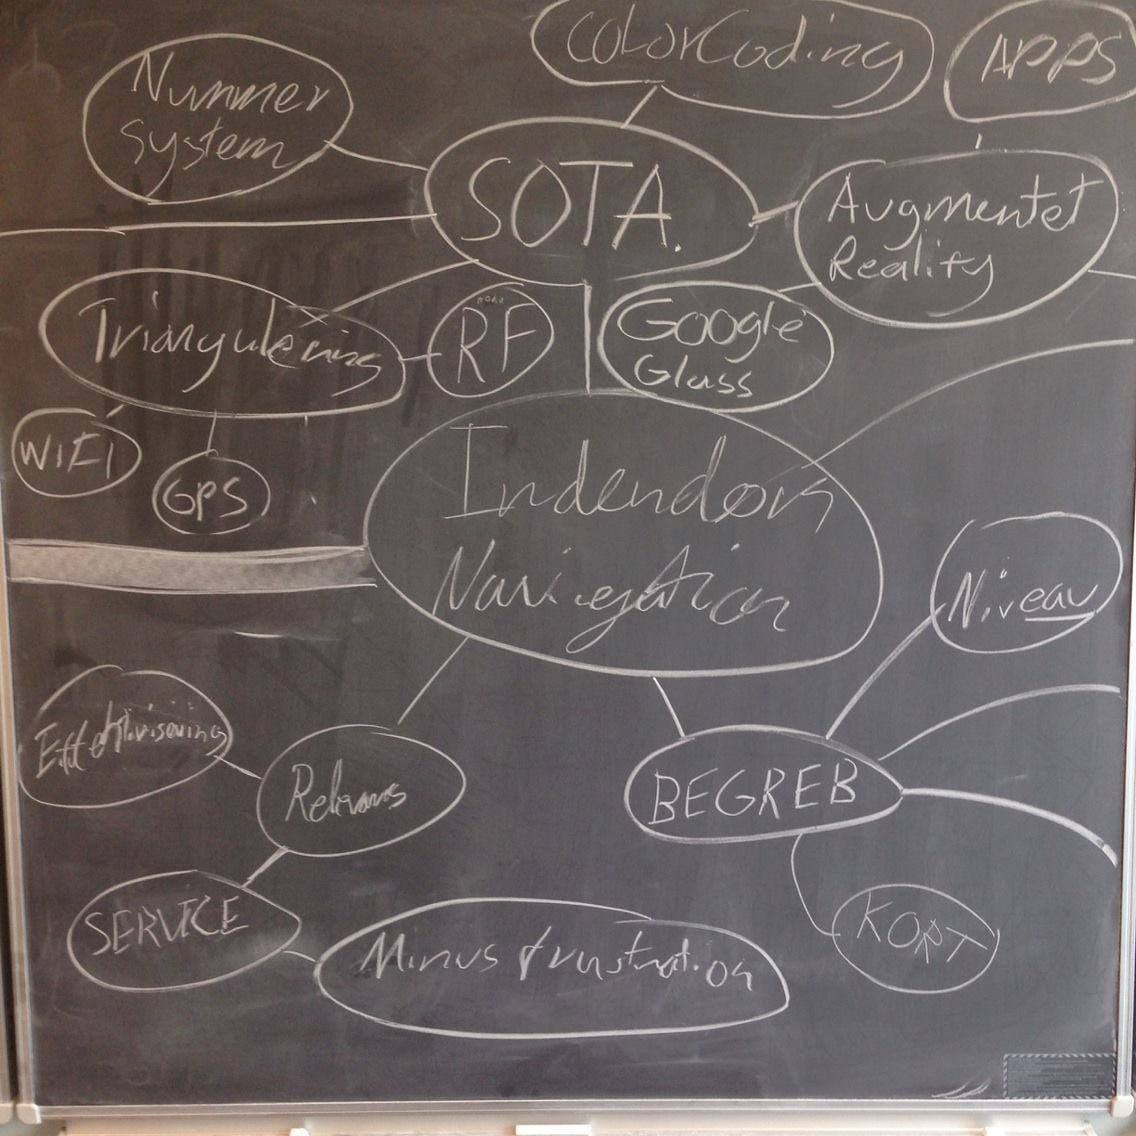
\includegraphics[width=\textwidth]{Images/4.jpg}
                \caption{BAH}
                \label{4}
            \end{minipage}
            \begin{minipage}{0.45\textwidth}
                \centering
                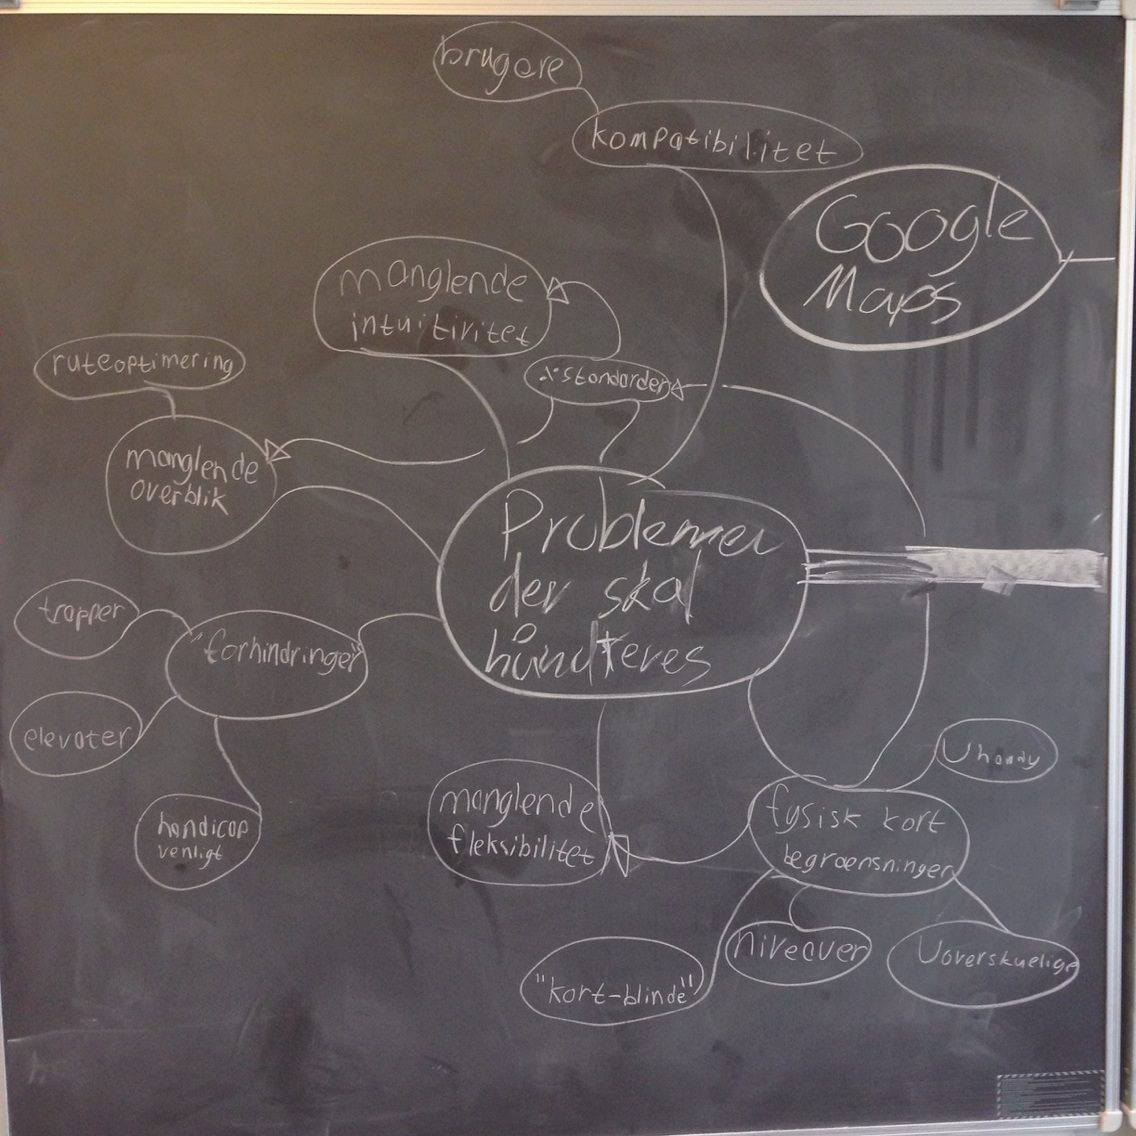
\includegraphics[width=\textwidth]{Images/7.jpg}
                \caption{BAH}
                \label{4}
            \end{minipage}
        \end{figure}

        \subsection{Tegninger}

Under mange af vores diskussioner, har vi illustreret det for gruppen på tavlen, så alle kunne være  med og her er et af ex. på vores diskussion omkring håndtering af "Floors", der er blevet lavet mange gode ting på tavlen, men ikke alle ting er der blevet taget billeder af.\newline

        \begin{figure}[ht!]
            \centering
            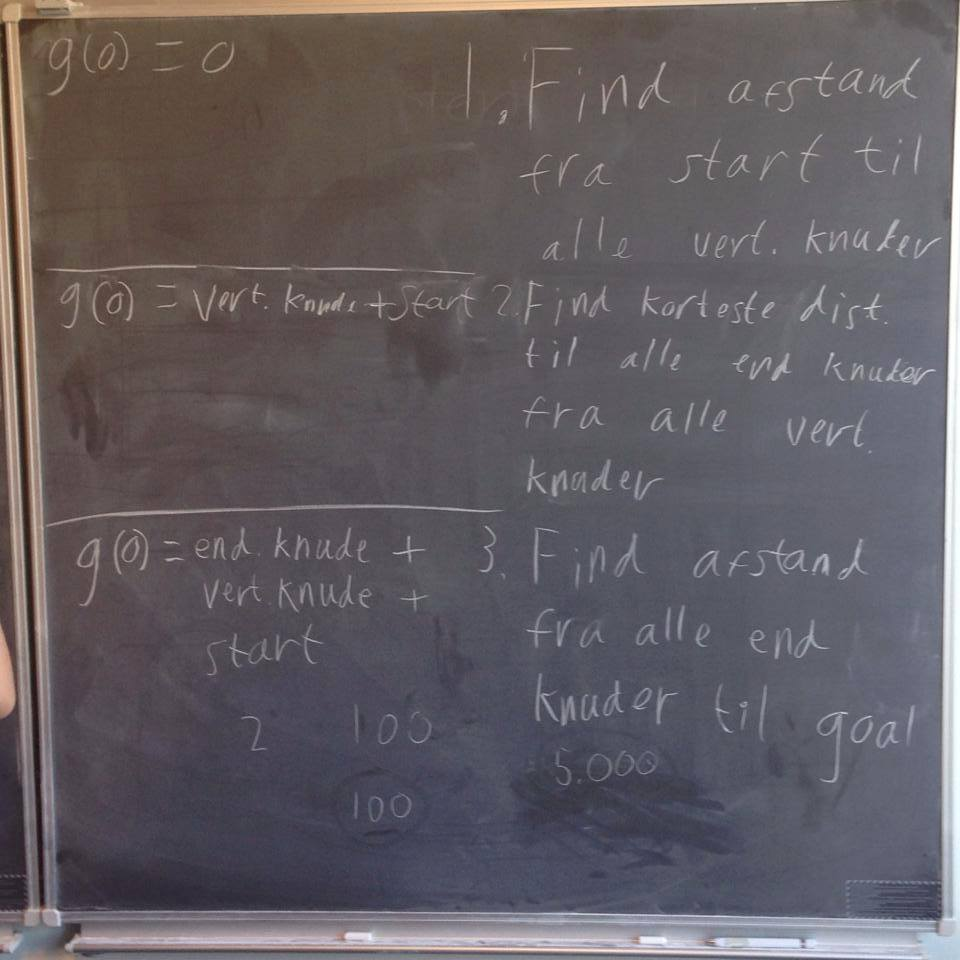
\includegraphics[width=0.5\textwidth]{Images/5.jpg}
            \caption{BAH}
            \label{4}
        \end{figure}

        \begin{figure}[ht!]
            \centering
            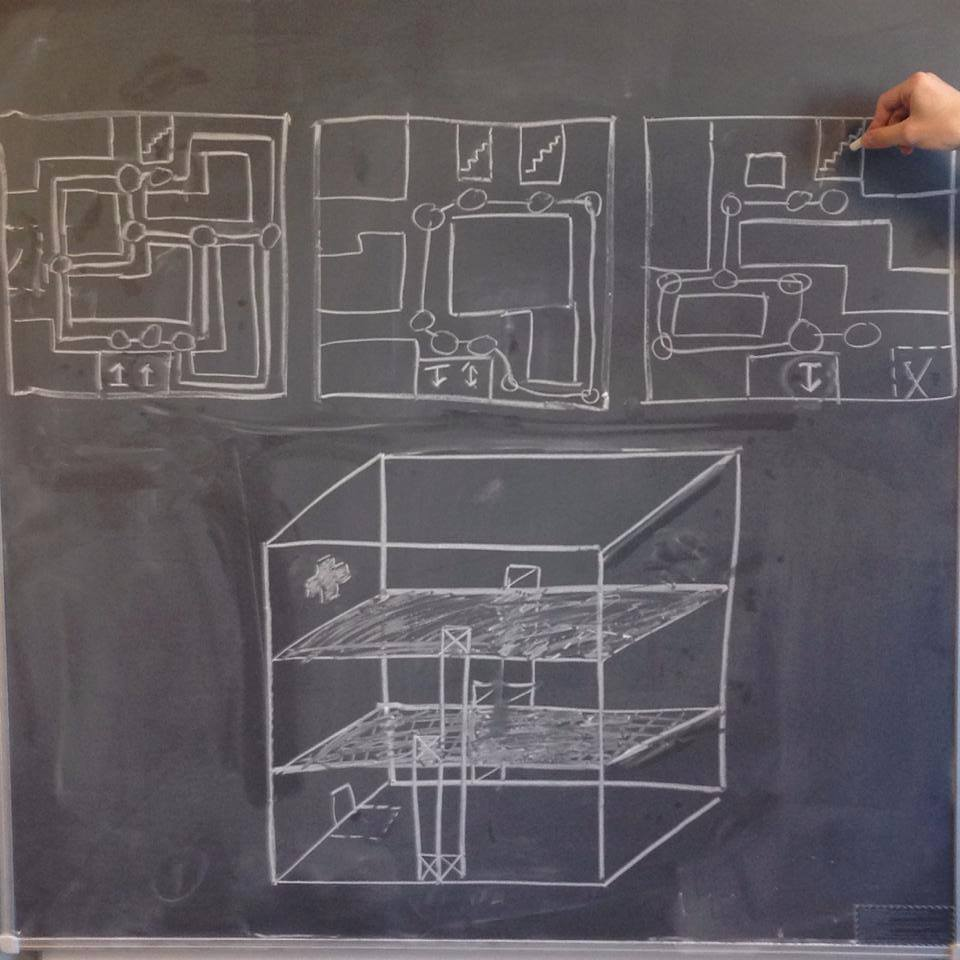
\includegraphics[width=0.5\textwidth]{Images/6.jpg}
            \caption{BAH}
            \label{4}
        \end{figure}

Hvilken argumentation brugte I for at motivere problemformuleringen?\newline
        
Hvad har I lært om hvordan problemformuleringer udarbejdes?\newline

        \subsection{Rapportstrukturering}

Hvordan bestemte I hvilke afsnit der skulle være i jeres P1 rapport?\newline

Hvordan bestemte I strukturen i rapporten?\newline

Hvordan sikrede I en rød tråd i rapporten?\newline

Hvilke afsnit havde I i jeres rapport, som I mener er generelle for alle projekter?\newline

    \section{Vurdering - Hvordan gik det}

Når I er færdige med at beskrive hvad I gjorde, skal I vurdere hvordan det gik. Med andre ord: Hvad gik godt i P1? Hvad gik dårligt i P1? \newline

    \section{Analyse - Hvorfor gik det som det gik}

Dernæst skal I analysere jeres arbejdsprocesser og få klarlagt hvorfor noget gik godt mens andet gik dårligt. Med andre ord: Hvad er det for faktorer, som har indvirket på arbejdsprocesserne? \newline

        
        \subsection{Andet}
- Under materialle læsning, sendte vi en gruppe ud på Syghus Nord Aalborg, for at tage billeder af hvordan navigeringen foregik, såsom farve kode, kort og skilte.\newline

    \section{Syntese - Gode råd til P2}

Hvis jeres vurdering og analyse skal bidrage til at forbedre jeres evne til at håndtere det problemorienterede og projektorganiserede gruppearbejde, skal I til slut konkretisere jeres erfaringer i nogle ’Gode råd’ til jer selv og jeres medstuderende. En god måde at formulere sådanne gode råd på er som en *start-stop-fortsæt*-liste, dvs. en liste med følgende tre sektioner: Dette vil vi begynde at gøre i P1, som vi ikke gjorde i P0 Dette vil vi ikke gøre i P1, som vi gjorde i P0 Dette vil vi fortsætte med at gøre (gerne anderledes og bedre) i P1, som vi også gjorde i P1.\newline

\end{document}